\documentclass{article}
\usepackage{amsmath}
\usepackage{amsfonts}
\usepackage{tikz}
\usepackage{qtree}
\usetikzlibrary{automata,arrows}

\begin{document}

\section*{Student Information}
Name: Batuhan Akçan \\
ID: 2580181 \\

\section*{Answer 1}
\subsection*{Part 1}
$K = \{s,p,q,f\}$\\
$\Sigma = \{a,b,\#\}$\\
$ \Gamma = \{a,b\} $\\
$\Delta = \{((s,a,e),(s,e)),\\
			((s,b,e),(s,e)),\\
			((s,e,e),(p,e)),\\
			((p,a,e),(p,a)),\\
			((p,b,e),(p,b)),\\
			((p,e,e),(q,e)),\\
			((q,a,e),(q,e)),\\
			((q,b,e),(q,e)),\\
			((q,\#,e),(f,e)),\\
			((f,a,a),(f,e)),\\
			((f,b,b),(f,e))\} $\vspace{0.1cm}\\
$s = s$\\
$F = \{f\}\vspace{0.3cm}$\\

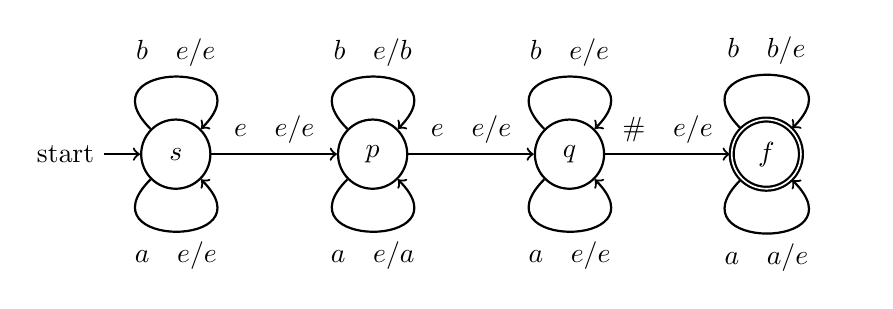
\begin{tikzpicture}[node distance={25mm}, thick, main/.style = {draw, circle}]
\node[initial,state] (1) {$s$};
\node[state] (2) [right of=1] {$p$};
\node[state] (3) [right of=2] {$q$};
\node[state,accepting] (4) [right of=3] {$f$};

\draw[->] (1) to [out=225,in=315,looseness=5] node[midway, below, sloped, pos=0.5] {$a \quad e/e$} (1);
\draw[->] (1) to [out=135,in=45,looseness=5] node[midway, above, sloped, pos=0.5] {$b \quad e/e$} (1);
\draw[->] (2) to [out=225,in=315,looseness=5] node[midway, below, sloped, pos=0.5] {$a \quad e/a$} (2);
\draw[->] (2) to [out=135,in=45,looseness=5] node[midway, above, sloped, pos=0.5] {$b \quad e/b$} (2);
\draw[->] (3) to [out=225,in=315,looseness=5] node[midway, below, sloped, pos=0.5] {$a \quad e/e$} (3);
\draw[->] (3) to [out=135,in=45,looseness=5] node[midway, above, sloped, pos=0.5] {$b \quad e/e$} (3);
\draw[->] (4) to [out=225,in=315,looseness=5] node[midway, below, sloped, pos=0.5] {$a \quad a/e$} (4);
\draw[->] (4) to [out=135,in=45,looseness=5] node[midway, above, sloped, pos=0.5] {$b \quad b/e$} (4);

\draw[->] (1) -- node[midway, above, sloped, pos=0.5] {$e \quad e/e$} (2);
\draw[->] (2) -- node[midway, above, sloped, pos=0.5] {$e \quad e/e$} (3);
\draw[->] (3) -- node[midway, above, sloped, pos=0.5] {$\# \quad e/e$} (4);

\end{tikzpicture}
\vspace{2.4cm}

\subsection*{Part 2}
$K = \{s,q,f\}$\\
$\Sigma = \{a,b,c\}$\\
$\Gamma = \{a,b,c\}$\\
$\Delta = \{((s,c,e),(s,c)),$\\
			$((s,e,e),(q,e)),$\\
			$((q,a,e),(q,a)),$\\
			$((q,b,e),(q,b)),$\\
			$((q,e,e),(f,e)),$\\
			$((f,a,a),(f,e)),$\\
			$((f,b,b),(f,e)),$\\
			$((f,c,c),(f,e))\}$\vspace{0.1cm}\\
$s = s$\\
$F = \{f\}$\vspace{0.3cm}\\

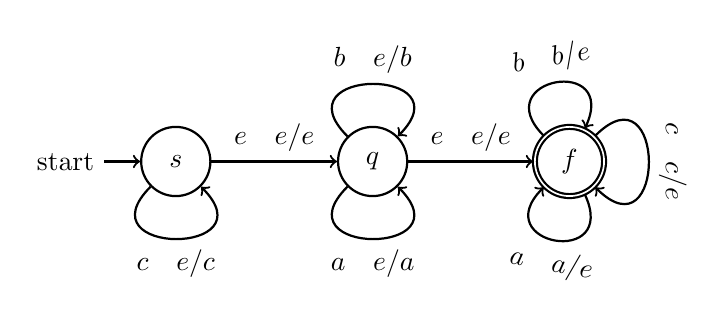
\begin{tikzpicture}[node distance={25mm}, thick, main/.style = {draw, circle}]
\node[initial,state] (1) {$s$};
\node[state] (2) [right of=1] {$q$};
\node[state,accepting] (3) [right of=2] {$f$};

\draw[->] (1) to [out=225,in=315,looseness=5] node[midway, below, sloped, pos=0.5] {$c \quad e/c$} (1);
\draw[->] (2) to [out=225,in=315,looseness=5] node[midway, below, sloped, pos=0.5] {$a \quad e/a$} (2);
\draw[->] (2) to [out=135,in=45,looseness=5] node[midway, above, sloped, pos=0.5] {$b \quad e/b$} (2);
\draw[->] (3) to [out=295,in=225,looseness=5] node[midway, below, sloped, pos=0.5] {$a \quad a/e$} (3);
\draw[->] (3) to [out=135,in=65,looseness=5] node[midway, above, sloped, pos=0.5] {$b \quad b/e$} (3);
\draw[->] (3) to [out=45,in=315,looseness=5] node[midway, above, sloped, pos=0.5] {$c \quad c/e$} (3);
\draw[->] (1) -- node[midway, above, sloped, pos=0.5] {$e \quad e/e$} (2);
\draw[->] (2) -- node[midway, above, sloped, pos=0.5] {$e \quad e/e$} (3);

\end{tikzpicture}

\section*{Answer 2}
Let $G = (V,\Sigma, R, S)$ where\\
$V = \{S,a,b\}$\\
$\Sigma = \{a,b\}$\\
$R = \{S \rightarrow SS,\; S \rightarrow aSa ,\; S \rightarrow bSb ,\; S \rightarrow aSb ,\;S\rightarrow bSa ,\; S \rightarrow e\}$\vspace{0.1cm}\\
Please have a look at the following parse tree:\\

\Tree[ .S [ .S a [ .S e ] a ] [ .S b [ .S a [ .S e ] b ] a ] ]\\

As you can see from the above tree, the resultant string $"aababa"$ is not a Kleene star of anything. So, adding the rule $S \rightarrow SS$ does not necessarily generate $L^*$.

\section*{Answer 3}
\subsection*{Part 1}
$L_1$ is a S-CFL because with $\Gamma = \{a\}$, the machine can recognize the language. Every time it reads $a$, it pushes $a$. Every time it reads $b$, it pops $a$.\\
$L_2$ is not a S-CFL because it needs to keep track of both the number of $a$'s
 and the number of $b$'s, so it needs 2 stack symbols.\\
$L_3$ is not a S-CFL because it needs to keep track of both the number of $a$'s
 and the number of $c$'s, so it needs 2 stack symbols.
\subsection*{Part 2}
$L = \{a^nbc^n \;|\; n \geq 0\}$\\
$G = \{V,\Sigma, R, S\}$ where\\
$V = \{S,a,b,c\}$\\
$\Sigma = \{a,b,c\}$\\
$R = \{S \rightarrow aSc,\; S \rightarrow b\}$
\subsection*{Part 3}
The memory element can be a counter.
\subsection*{Part 4}
There is only one stack symbol. The counter counts the number of occurences of that stack symbol. When the stack symbol is pushed, the value in the counter is incremented by 1. When the stack symbol is popped, the value in the counter is decremented by 1. For example, have a look at $L_1$ at part 1. While the machine is reading the given string, whenever it reads an $'a'$, the value at the counter will be incremented by 1. Whenever it reads a $'b'$, the value at the counter will be decremented by 1. When counter becomes 0, the machine terminates. In this way, S-PDAs can be implemented with a counter.
\subsection*{Part 5}
No. Have a look at the $L_1$ at part 1. Let the complement of it be $L_1'$. Then $L_1'$ must include the set of strings $\{a^nb^{n+2} \;|\; n \geq 0\}$. With a single stack element, the machine can not know how many $b$'s it should read after reading $n$ number of $a$'s. It will read $n$ number of $b's$, but, after that, since the stack is empty, it can not know that it should read 2 more $b$'s. That's why, the class of S-CFLs is not closed under complementation.






\end{document}